\section{Architektura systemu}
\label{chat_architektura_systemu}

Architektura systemu opiera się na klasycznym modelu klient-serwer.

Klienci będą uzyskiwali dostęp do usługi czatu za pośrednictwem przeglądarki
internetowej. Łącząc się z podanym adresem (IP lub domeny), na którym połączeń
nasłuchuje serwer, w pierwszej kolejności przeglądarka będzie próbować połączyć
się z nim przy użyciu protokołu http i standardowego portu 80, wysyłając do
niego żądanie metodą GET. Wówczas, serwer będzie zawsze odpowiadał statycznym
plikiem HTML, zawierającym odwołania do skryptów w języku JavaScript (JS) oraz
pozostałej, statycznej treści (np. grafiki czy arkusze stylów CSS). Serwer
będzie odsyłał te pliki do przeglądarki w odpowiedzi na kolejne żądania HTTP
GET, wysyłane w miarę dalszego renderowania pliku HTML. W ten sposób, po
stronie klienta zostanie pobrana i uruchomiona aplikacja internetowa typu
Single Page
Application, której interfejs będzie reagował z użytkownikiem oraz ulegał
zmianom wskutek działania skryptów JS, załadowanych na pierwszym etapie
uruchomienia. Po stronie serwera, dostarczaniem treści statycznych będzie
zajmował się daemon HTTP - Nginx.

Gdy tylko skrypty JS wykryją pobranie wszystkich plików składowych aplikacji
z serwera, podjęta zostanie próba nawiązania połączenia z tym serwerem przy
użyciu protokołu WebSocket. Będzie on od tego momentu podstawowym kanałem
komunikacji pomiędzy klientem a serwerem.

Zgodnie ze standardem WebSocketu, zanim zostanie nawiązane właściwe połączenie,
powinno dojść do „uścisku dłoni” (ang. \textit{handshake}) pomiędzy klientem a
serwerem. W związku z tym, pierwsza próba połączenia również zostanie podjęta
przy użyciu protokołu http, jednakże tym razem pod innym, dedykowanym portem
(w naszym przypadku będzie to port 8000), a także zawierać nagłówki wskazujące
na żądanie zmiany używanego protokołu na WebSocket, jego wersję oraz klucz
(„Sec-WebSocketKey”). Serwer udzieli wówczas odpowiedzi ze swoim własnym
kluczem, informując o zmianie stosowanego protokołu na WebSocket.

W chwili prawidłowego rozpoczęcia połączenia WebSocket, aplikacja po stronie
klienta wyświetli użytkownikowi okno autoryzacyjne. Wpisane tam dane zostaną
następnie przesłane do serwera. Po jego stronie, komunikat zostanie zdekodowany
przez aktora \texttt{WSConnector} i przekazany powiązanemu aktorowi
\texttt{Authorizer}. Jego zadaniem będzie weryfikacja przedstawionych informacji
oraz podjęcie decyzji o autoryzacji lub jej odmowie. Decyzja ta jest odsyłana do
\texttt{WSConnectora} i następnie przekazywana do aplikacji po stronie klienta.

Jezeli autentykacja przebiegnie pomyślnie, aktor \texttt{Authorizer} uruchamia
aktora \texttt{UserSession}, spina go z aktorem \texttt{WSConnector} używanym
wcześniej do komunikacji z frontendem, oraz ulega autodestrukcji.

\newpage

\subsection{Dekompozycja systemu na podsystemy}
\label{architektura_chatu}

\subsubsection{Strona serwera (,,backend'')}
Na serwer czatu składa się grupa współdziałających, ale zupełnie odrębnych od siebie aktorów.

\begin{figure}[!htp]
	\centering
	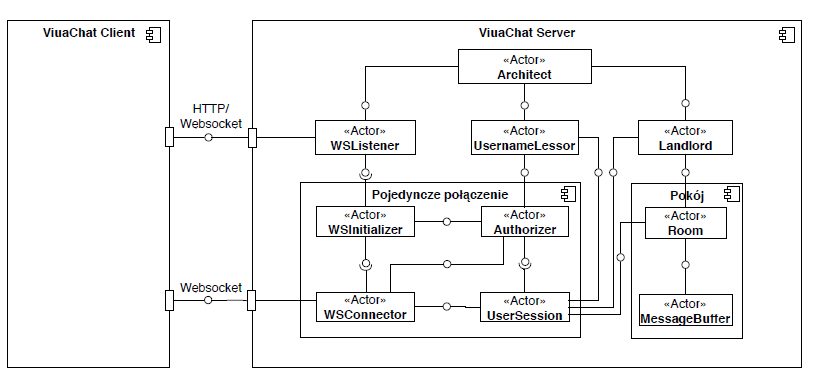
\includegraphics[width=\textwidth]{chat/fig/pck-diag}
	\caption{Diagram komponentów serwera ViuaChat}
	\label{diag-komp}
\end{figure}

\begin{figure}[!htp]
	\centering
	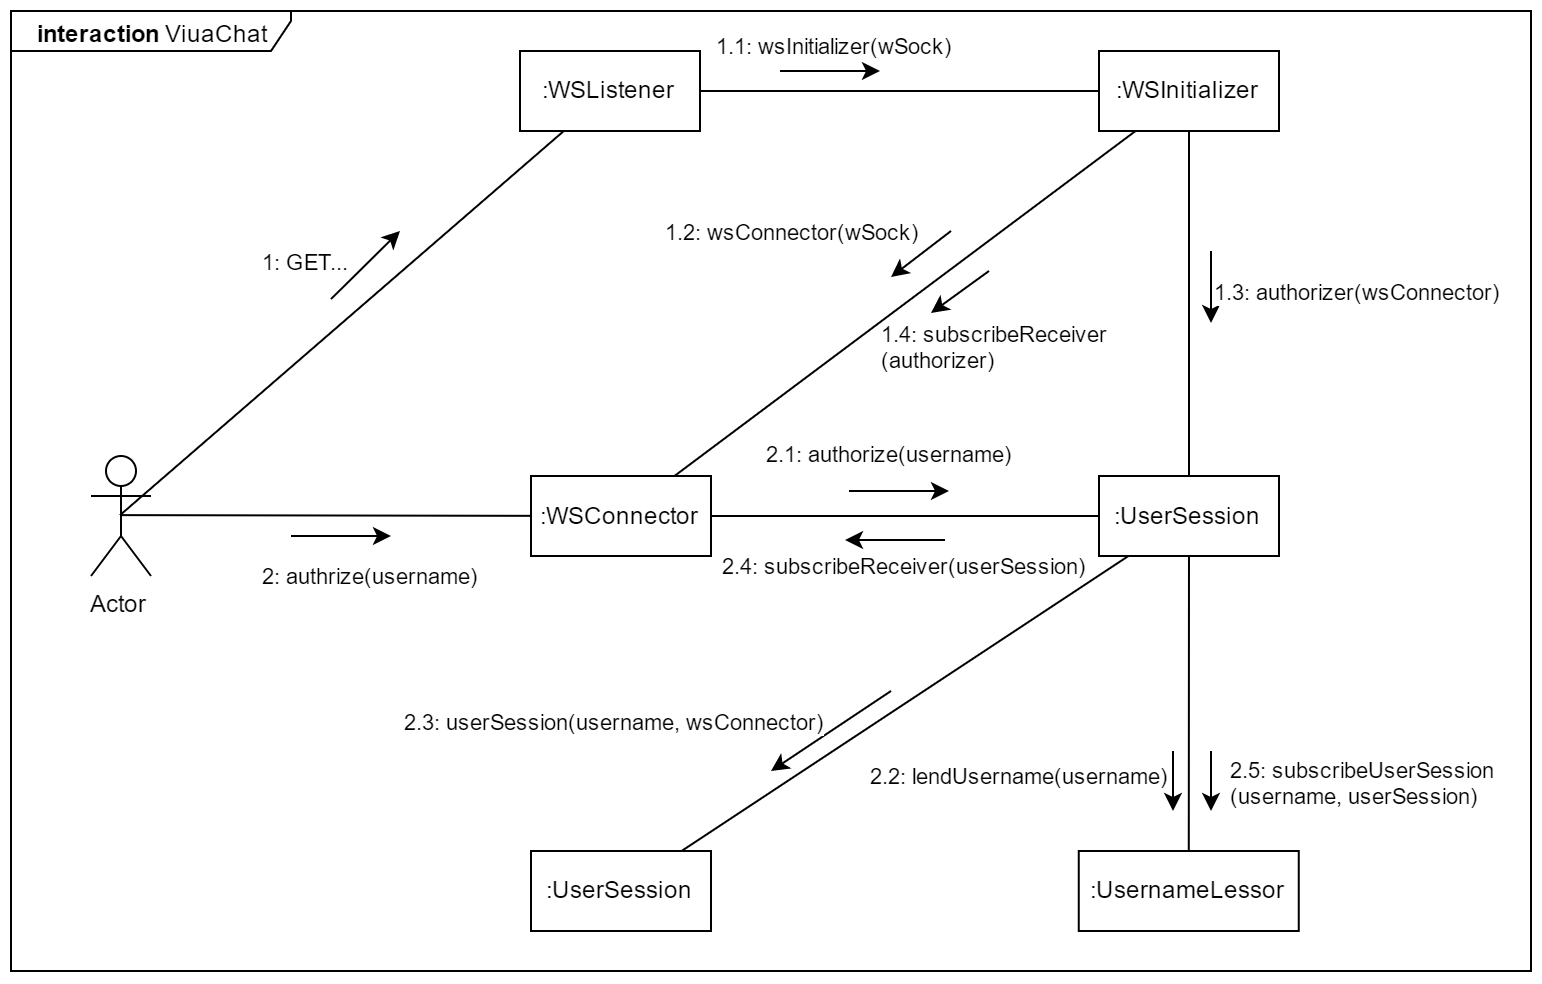
\includegraphics[width=\textwidth]{chat/fig/com-diag-init}
	\caption{Diagram komunikacji pomiędzy aktorami w czasie nawiązywania połączenia}
	\label{com-diag-init}
\end{figure}

\begin{labeling}{UsernameLessor}

  \item[\texttt{Architect}] Uruchamiany jako pierwszy wraz z całym
  serwerem, a następnie inicjalizuje i nadzoruje aktorów \texttt{WSListener},
  \texttt{UsernameLessor} oraz \texttt{Landlord}. W razie nieprawidłwego
  działania lub wyłączenia któregokolwiek z tych trzech głównych aktorów,
  \texttt{Architect} automatycznie zainicjuje przeładowanie całego serwera.
  Ponadto, \texttt{Architect} potrafi w momencie uruchamiania serwera odczytać
  jego pliki konfiguracyjne i na tej podstawie należycie skonfigurować pokoje
  oraz administratorów. Zawsze występuje w jednym egzemplarzu.

  \item[\texttt{WSListener}] Odpowiada za nasłuchiwanie na porcie 8000 po
  stronie serwera, a przy każdej próbie połączenia będzie tworzyć kolejnego,
  niezależnego aktora \texttt{WSInitializer}. Występuje zawsze w jednym
  egzemplarzu.

  \item[\texttt{WSInitializer}] Odpowiada za  realizację ,,uścisku dłoni'' i
  formułowanie odpowiedzi zwrotnej po stronie serwera w odniesieniu do
  połączenia na konkretnym gnieździe. W razie prawidłowego nawiązania
  połączenia, aktor ten utworzy kolejną parę aktorów, \texttt{WSConnector} oraz
  \texttt{Authorizer}, zaś WSInitializer ulegnie samozniszczeniu.

  \item[\texttt{WSConnector}] Odpowiada za dalszą, bezpośrednią obsługę
  przydzielonego gniazda. Występuje ich tylu, ile jest otwartych połącznień.
  Jego rolą będzie również kodowanie i dekodowanie wiadomości (ang.
  ,,messages''), czyli podstawowych logicznych jednostek informacji, które są
  używane przy połączeniach z użyciem protokołu WebSocket. Pilnuje również, czy
  połączenie nie zostało zerwane oraz inicjuje zamykanie sesji użytkownika.

  \item[\texttt{Authorizer}] Wymienia wiadomości od \texttt{WSConnectora}, który
  został uruchomiony wraz z nim i odpowiada za należytą autentykację i/lub
  autoryzację użytkownika w usłudze czatu. Egzemplarz aktora tego typu jest
  powoływany dla każdego otwartego połączenia bez nawiązanej sesji. Aby dokonać
  autoryzacji, aktor \texttt{Authorizer} kontaktuje się \texttt{UsernameLessor}.
  Jeżeli autentykacja przebiegnie pomyślnie, aktor \texttt{Authorizer} uruchamia
  aktora \texttt{UserSession}, spina go z aktorem \texttt{WSConnector} używanym
  wcześniej do komunikacji z frontendem, oraz ulega autodestrukcji.

  \item[\texttt{UsernameLessor}] Jego zadaniem jest zarządzanie informacjami na
  temat tymczasowych nazw użytkowników, należących do	użytkowników bez stałych
  kont (ich gromadzenie, udzielanie, weryfikacja, dbanie o unikalność), a także
  weryfikacja tożsamości kont administratorów z dodatkowym użyciem hasła.
  Występuje w jednym egzemplarzu, przez cały czas istnienia serwera. Ponadto,
  nadzoruje działanie aktorów \texttt{Authorizer} oraz \texttt{UserSession}.

  \item[\texttt{UserSession}] Przejmuje komunikację z użyciem
  \texttt{WSConnector}, pozwalając na zwyczajne użytkowanie czatu. Aktor
  ,,UserSession'' gromadzi informacje na temat nazwy oraz poziomu uprawnień
  użytkownika, a także tego, z jakim pokojem jest obecnie spięty.

  \item[\texttt{Landlord}] Jego zadaniem jest współudział w podpinaniu
  użytkowników do pokoju, tworzeniem nowych i usuwaniem istniejących pokojów, a
  także utrzymywanie i udostępnianie kompletnej listy aktywnych pokojów.

  \item[\texttt{Room}] Działa jak router wiadomości i przechowuje listę użytkowników którzy są do niego wpięci. Istnieje w tylu egzemplarzach, ile jest aktywnych pokojów.

  \item[\texttt{MessageBuffer}] Przechowuje i odtwarza 10 najnowszych wiadomości wysłanych do pokoju. Występuje po jednym egzemplarzu dla każdego aktywnego aktora \texttt{Room}.

\end{labeling}

\newpage

\subsubsection{Warstwa interfejsu użytkownika (,,frontend'')}
Podczas pracy nad wartwą frontendu, zastosowano framework webowy Vue.js. Jedną
z przyczyn dla tej decyzji jest możliwość zdekomponowania projektowanej aplikacji na mniejsze części, nazywane modułami (ang. \textit{modules}). Są one zorganizowane hierarchiczne. Każdy z modułów zawiera własny skrypt JavaScript, a także kod HTML i arkusz CSS. Powoduje to, że każdy z modułów jest niezależny od pozostałych i może realizować swoje zadania w pełni autonomicznie.

Każdy z modułów udostępnia swojemu rodzicowi pewne określone parametry. Ich zmiana
jest podstawowym sposobem na interakcję pomiędzy nimi, co jest zgodne z
paradygmatem \textit{data driven application} (z ang. ,,aplikacja sterowana
poprzez dane''). W podobny sposób następuje zmiana kodu HTML modułów. Zamiast
zmieniać węzły DOM w sposób jawny poprzez skrypt, programista wskazuje w
szablonie HTML te miejsca, które ulegają określonym przemianom wraz ze
zmian wewnętrznych parametrów modułu.

Podstawowa struktura aplikacji frontendowej przewiduje podział na
pięć części:
\begin{itemize}
	\item Część autoryzacyjna -- służy do nawiązania połączenia z
	serwerem i rozpoczęcie sesji użytkownika.

	\item Pokoje (publiczne) -- dostarcza listę ogólnodostępnych pokojów,
	umożliwia podpięcie się wybranych z nich oraz prowadzenie rozmów z
	innymi użytkownikami, którzy się do nich podpięli.

	\item Wiadomości prywatne -- umożliwia nawiązywanie prywatnych
	rozmów pomiędzy użytkownikami oraz wymianę wiadomości prywatnych.

	\item Narzędzia administracyjne -- pozwalają administratorom
	na dodawanie i usuwanie pokojów, wyrzucanie użytkowników z pokojów
	i z serwera.

	\item Profil użytkownika -- umożliwia podejrzenie informacji na
	temat własnego konta, zmianę przez administratora swojego hasła
	użytkownika oraz rozłączenie się z serwerem.

\end{itemize}

W projekcie przewidziano zastosowanie modułów, przedstawionych na rysunku \ref{diag-komp-front}.

\nameref{diag-komp-front}.
\begin{figure}[!htp]
	\centering
	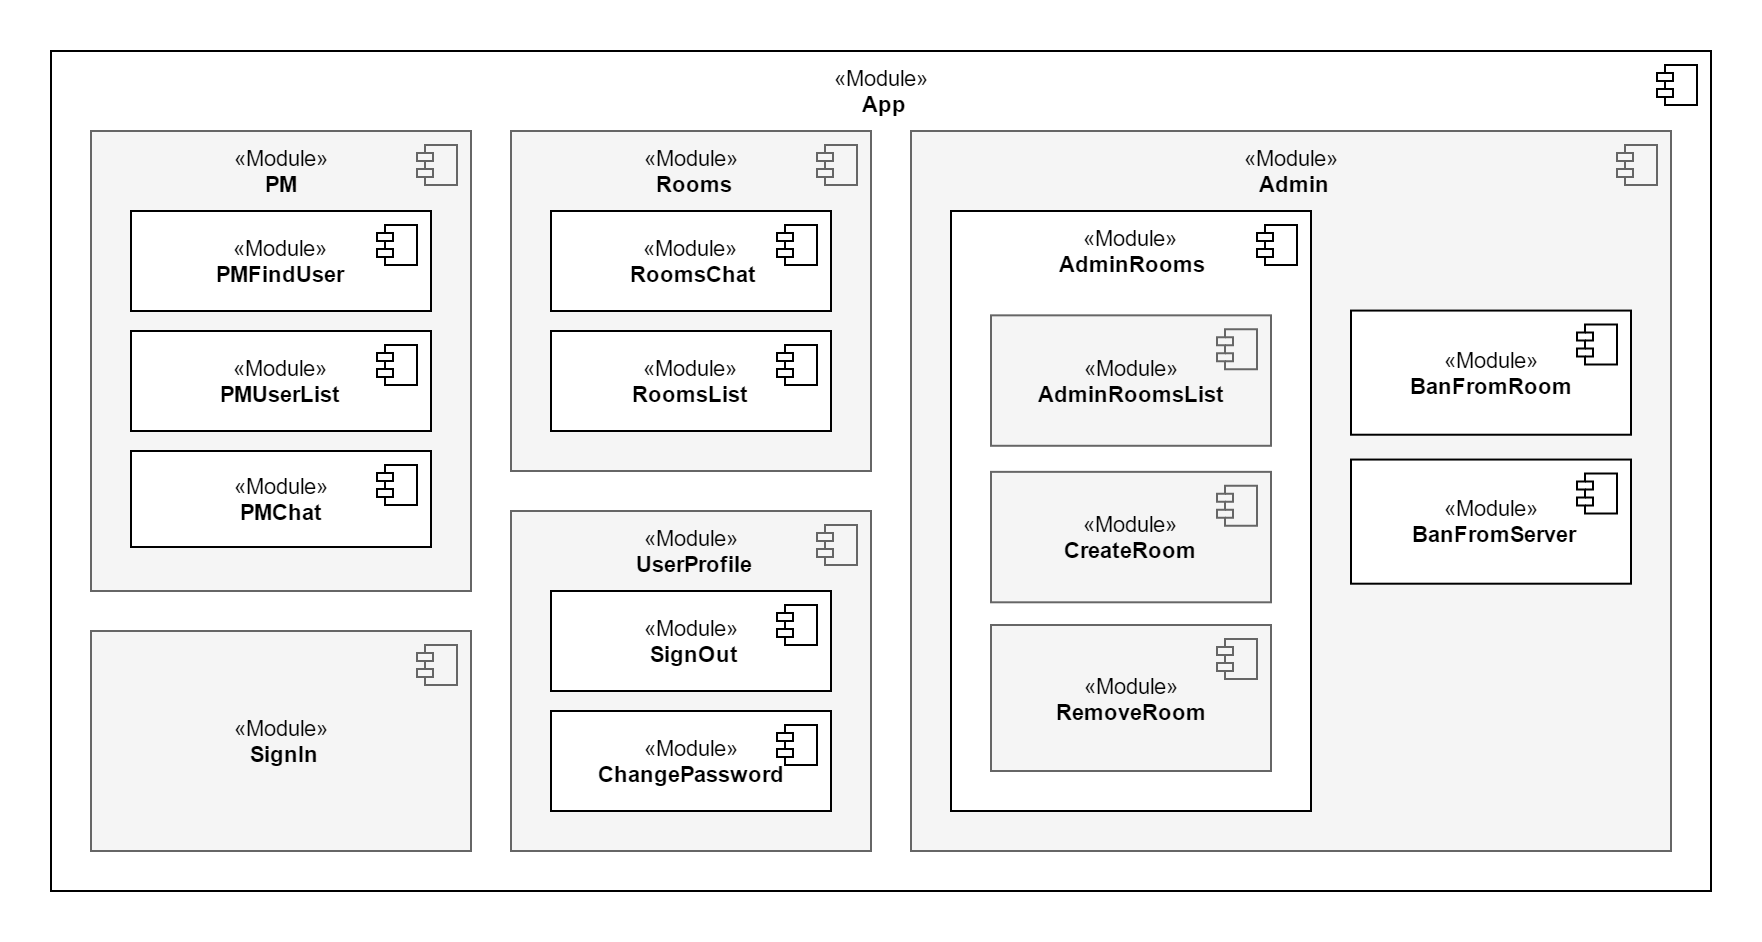
\includegraphics[width=\textwidth]{chat/fig/pck-diag-front}
	\caption{Diagram komponentów aplikacji webowej ViuaChat}
	\label{diag-komp-front}
\end{figure}

\begin{labeling}{\texttt{UserProfile}}

  \item[\texttt{App}] Nadrzędny moduł, istniejący przez cały czas użycia
	instancji aplikacji. Obejmuje najbardziej zewnętrzne struktury HTML,
	przechowuje podstawowy stan aplikacji (stan autoryzacji, nazwę
	użytkownika, poziom uprawnień, gniazdo WebSocket dla połączeń
	z wartwą backendu), a także zapewnia routing do głównych części
	aplikacji - czyli modułu logowania, modułu pokojów (publicznych),
	pokojów prywatnych wiadomości, profilu użytkownika i narzędzi
	administracyjnych.

	\item[\texttt{SignIn}] Moduł odpowiadający za początkową autoryzację
	do serwera (potocznie znane jako ,,logowanie'').

	\item[\texttt{Rooms}] Moduł reprezentuje część aplikacji poświęconą
	ogólnodostępnym pokojom dla wspólnych konwersacji. Podlegają mu:

	\begin{labeling}{\texttt{RoomsChat}}
		\item[\texttt{RoomsChat}] Moduł odpowiedzialny \textit{stricte} za
		okno czatu - wyświetlanie konwersacji oraz wysyłanie wiadomości
		do pokoju.

		\item[\texttt{RoomsList}] Moduł wyświetlający listę pokojów, a także
		umożliwiający podpięcie się do wybranego z nich.

	\end{labeling}

	\item[\texttt{PM}] Moduł odwzorowujący całą część aplikacji poświęconą
	wymianie pomiędzy użytkownikami wiadomości prywatnych. W jego skład
	wchodzą:

	\begin{labeling}{\texttt{PMUserList}}
		\item[\texttt{PMFindUser}] Moduł, którego zadaniem jest odnalezienie
		użytkowika, do którego ma zostać wysłana wiadomość prywatna

		\item[\texttt{PMUserList}] Moduł obsługujący listę użytkowników,
		którzy wcześniej otrzymali lub wysłali wiadomości prywatne.

		\item[\texttt{PMChat}] Moduł odpowiedzialny za obsługę zasadniczego
		okna czatu wiadomości prywatnych, pozwalającego wymieniać wiadomości
		prywatne z jednym, wybranym użytkownikem.
	\end{labeling}

\item[\texttt{UserProfile}] Moduł pozwalający na podstawową kontrolę
własnego profilu, w tym:

\begin{labeling}{\texttt{ChangePassword}}
	\item[\texttt{SignOut}] Moduł odpowiedzialny za zamknięcie sesji
	użytkownika, rozłączenie z serwerem oraz powrót aplikacji do
	stanu sprzed autoryzacji

	\item[\texttt{ChangePassword}] Moduł mający umożliwiać administratorom
	zmianę swoich własnych haseł

\end{labeling}

\item[\texttt{Admin}] Moduł obejmujący pod sobą wszystkie narzędzia
administracyjne. W jego skład wchodzą:

\begin{labeling}{\texttt{BanFromServer}}
	\item[\texttt{AdminRooms}] Moduł do zarządzania ogólnodostępnymi
	pokojami czatu, w tym:

	\begin{labeling}{\texttt{AdminRoomsList}}
		\item[\texttt{AdminRoomsList}] Moduł listy wszystkich ogólnodostępnych
		pokojów z narzędziami do ich edycji

		\item[\texttt{CreateRoom}] Moduł pozwalający na dodawanie pokojów
		do serweru czatu

		\item[\texttt{RemoveRoom}] Moduł pozwalający na usuwanie istniejących
		pokojów z serwera
	\end{labeling}

	\item[\texttt{BanFromRoom}] Moduł służący do wyrzucania użytkowników
	z pokojów, w których obecnie się znajdują.

	\item[\texttt{BanFromServer}] Moduł pozwalający na wyrzucenie
	użytkowników z serwera.
\end{labeling}

\end{labeling}
\section{Decyzje projektowe}

\subsection{Środowisko docelowe}
Decyzje związane ze środowiskiem docelowym zostały zdeterminowane w głównej
mierze przez wymagnia WS-01, WS-02 i WS-03. Punktem wyjścia była konieczność
uruchomienia serwera czatu (backendu) na maszynie Viua VM. W związku z tym,
z kręgu zaintersowań wypadły systemy operacyjne z rodziny Windows, z uwagi na
ich niekompatybilność z Viua VM. Wybór padł na system operacyjny Linux Mint,
ponieważ jest dobrze utrzymywaną platformą opartą o Debiana. Ważkim argumentem
była łatwość obsługi tej dystrybucji przez nowych użytkowników, którzy nie byli zaznajomieni wcześniej z rozwiązaniami linuksowymi.

W dalszej kolejności należało podjąć decyzję, w jaki sposób serwować pliki
związane z warstwą frontendu. Propozycja użycia serwera Nginx została uznana
za słuszną. Zespół przekonała prostota tego rozwiązania. Równocześnie, serwer
Nginx był serwerem wypróbowanym i rozwijanym od wielu lat. Uznano zatem, że
będzie użyteczny również w środowisku produkcyjnym.

Na cele obrony pracy dyplomowej, przygotowano i uruchomiono serwer wirtualny u
dostawcy usług chmurowych, aby zapewnić niezależność od infrastruktury na
miejscu prezentacji i zapewnić jej należyty poziom niezawodności. Nie jest
on jedak niezbędny do uruchomienia aplikacji przez potencjalnego, przyszłego
użytkownika platformy \ViuAct.

Aby zademonstrować możliwości wielowątkowości w praktyce, urządzenie docelowe,
na którym przyszły użytkownik będzie uruchamiał serwer czatu, powinno dysponować
wielordzeniowym procesorem. Nie ma tu znaczenia, w jakiej architekturze
zrealizowano określony procesor. Za uruchamianie poszczególnych wątków odpowiada
bowiem Viua VM.

Urządzenia, które mają zaprezentować funkcjonowanie systemu w wykorzystaniu
przez użytkowników końcowych, to komputery przenośne (laptopy), jeden z systemem
operacyjnym Windows 10, a drugi -- z zainstalowaną dystrybucją Linux Mint, o
której wspomniano wcześniej w kontekście środowiska wytwórczego. Zaplanowano
również wykorzysanie dwóch urządzeń mobilnych. Jedno z nich jest tabletem z
rodziny Samsung Galaxy, a drugim -- smartfon LG K11. Oba z nich są wyposażone
w dystrybucje systemu operacyjnego Android oraz przeglądarkę Google Chrome.
Dodanie urządzeń mobilnych do zestawu demonstracyjnego ma przede wszystkim
uczynić zadość wymaganiu WS-03.

\subsection{Środowisko implementacji}
Pierwszym kryterium przy doborze składników środowiska implementacyjnego była
spójność z rozwiązaniami produkcyjnymi. Miało to pozwolić uniknąć problemów
z przenośnością. Na środowisko implementacyjne wybrano laptop z takim samym
systemem operacyjnym, w jakim ma być uruchomiona ViuaVM wraz z oprogramowaniem
serwera czatu. Szczegółowo, warstwę sprzętowo opisano w \fullref{existing-infr}.

Jak już wspomniano, nie jest możliwe skompilowanie i uruchomienie Viua
VM w systemach Microsoft Windows. W związku z tym, początkowo serwer był
uruchamiany po systemem operacyjnym Linux Mint, zainstalowanym na maszynie
wirtualnej uruchomionej w środowisku Oracle VirtualBox. Gdy pierwsze testy
uruchomieniowe zostały zakończone z powodzeniem, pracę nad projektem
przeniesiono na komputer z natywnie zainstanowanym systemem Linux Mint.

Równolegle z testami współpracy Viua VM ze środowiskiem Linux Mint, Marek
Marecki przygotowywał skrypt powłoki Bash oraz zestaw repozytoriów Git z
podstawowymi komponentami platformy \ViuAct\ (czyli maszyną Viua VM, kompilatorem
\ViuAct i kolekcją bibliotek zewnętrznych). Tak przygotowany zestaw mógł zostać
pobrany i skompilowany z użyciem jednej komendy, co znacznie ułatwiło prace
nad czatem.

\section{Projekt algorytmów i przyjętych protokołów}

\subsection{Protokół frontend-backend}
Komunikacja pomiędzy frontendem a backendem będzie odbywać się poprzez wymianę
krótkich komunikatów tekstowych, opisujących struktury danych w standardzie
JSON. Przyjęto, że komunikaty dzielą się na dwie grupy:

\begin{enumerate}
	\item \textbf{Synchroniczne} -- są wysyłane zawsze od klienta do serwera, a
	serwer zawsze odpowiada na nie klientowi, podając informację na temat
	powodzenia żądanej operacji lub też przesyłając oczekiwane dane.

	\item \textbf{Asynchroniczne} -- mogą być wysyłane z inicjatywy dowolnej ze
	stron i nie są związane z obowiązkiem jakiejkolwiek odpowiedzi.
\end{enumerate}

\subsubsection{Budowa komunikatów synchronicznych}
Prawidłowe komunikaty synchroniczne, wysyłane przez klienta do serwera, mają
następującą budowę:
\begin{lstlisting}
  {
    'fn': 'funkcja',
    'arg':
    {
      'argument1' : 123,
      'argument2' : 'abc'
    },
    'seq': 1,
		'session_key': 'abcdef123456'
  }
\end{lstlisting}

Kolejne własności obiektu, wyrażonego w notacji JSON:
\begin{itemize}
	\item \texttt{fn} -- łańcuch znaków, który wskazuje, jakiej funkcjonalności
	(operacji) dotyczy wysłany komunikat (np. \texttt{auth} przy autoryzacji
	lub \texttt{bind\_room} przy podpinaniu użytkownika do pokoju);

	\item \texttt{arg} -- obiekt, który przenosi dodatkowe argumenty niezbędne do
	realizacji żądanej operacji (np. np. login i hasło przy komunikacie autoryzacji na
	serwer lub nazwę pokoju przy komunikacie podpięcia); obiekt ten może zawierać jedynie
	parametry z typami prostymi, takimi jak łańcuchy znaków czy liczby całkowite;
	parametr \texttt{arg} jest obowiązkowy ale zawarta w nim struktura może być
	pusta \texttt{/{/}};

	\item \texttt{seq} -- numer kolejny komunikatu, generowany po stronie klienta,
	który pozwoli mu potem zorientowac się, na jaki komunikat została przesłana
	konkretna odpowiedź serwera;

	\item \texttt{session\_key} -- łańcuch znaków, będący kluczem sesji, przy użyciu
	którego użytkownik autoryzuje wiadomość; klucz jest uzyskiwany przy autoryzacji
	do serwera; parametr \texttt{session\_key} nie jest obowiązkowy dla wiadomości typu
	\texttt{auth} przed uzyskaniem pozytywnej autoryzacjji;
\end{itemize}

Budowa komunikatu, będącego odpowiedzią serwera na komunikat synchroniczny,
zależy od powodzenia żądanej operacji. W razie sukcesu wygląda następująco:

\begin{lstlisting}
{
  'seq': 1,
  'result': 1,
  'par':
  {
    'parametr1': 123,
    'parametr2': 'abc'
  }
}
\end{lstlisting}

Z kolei, w przypadku błędu po stronie serwera, komunikat wygląda następująco:

\begin{lstlisting}
{
  'seq': 1,
  'result': 0,
  'par': {},
  'error_code': 101,
  'error_name': 'Brak uprawnien'
}
\end{lstlisting}

Poniżej wskazano, jakie typy i znaczenia mają kolejne własności obiektu w
notacji JSON:
\begin{itemize}
	\item \texttt{seq} -- liczba całkowita, przepisana z wiadomości od klienta,
	pozwalająca zorientować się, jakiej komendy dotyczy wysłany komunikat.

	\item \texttt{result} -- licba całkowita 1 lub 0, która wskazuje, czy żądana
	operacja została zakończona powodzeniem (1 oznacza sukces, a 0 wskazuje na
	błąd);

	\item \texttt{par} -- obiekt, który przenosi dodatkowe parametry z danymi,
	których mógł żądać użytkownik (np. listę nazw pokojów podczas logowania);
	dokładna struktura obiektu zależy od tego, jakiego typu była żądana
	operacja; parametr \texttt{par} jest obowiązkowy przy odpowiedziach, ale
	zawarty w nim obiekt może być pusty \texttt{\{\}}; schmeat

	\item \texttt{error\_code} -- liczba całkowita będąca kodem identyfikującym błąd, który wystąpił po stronie serwera podczas wykonywania żądanej operacji; parametr pojawia się wyłącznie wówczas, gdy wykonanie operacji zakończyło się niepowodzeniem;

	\item \texttt{error\_name} -- łańcuch znaków opisujący błąd, który wystąpił
	po stronie serwera podczas wykonywania żądanej operacji; parametr pojawia
	się wyłącznie wówczas, gdy wykonanie operacji zakończyło się niepowodzeniem;

\end{itemize}

\subsubsection{Typy komunikatów synchronicznych}

\leavevmode\hbox{}

{\footnotesize
\begin{longtable}{ | l | l | l | l | l | }
\hline
	\textbf{Lp} &
	\textbf{Typ (\texttt{fn})} &
	\parbox{3.9cm}{\textbf{Nazwa funkcjonalności (operacji)}} &
	\parbox{3.9cm}{\textbf{Oczekiwane argumenty (\texttt{arg})}} &
	\parbox{3.9cm}{\textbf{Oczekiwane parametry odpowiedzi (\texttt{par})}}
	\\

	\hline
		\parbox[t]{0.8cm}{
			1

		} & \parbox[t]{1.7cm}{\strut
			\texttt{auth}

		\strut} & \parbox{4.1cm}{
			Autoryzacja do czatu

		} & \parbox{3.9cm}{
			\begin{itemize}
				\item \texttt{username} (nazwa użytkownika);
				\item \texttt{password} (hasło)
			\end{itemize}


		} & \parbox{3.9cm}{
			\begin{itemize}
				\item \texttt{session\_key} (klucz sesji)
			\end{itemize}
		} \\

	\hline

	\parbox[t]{0.8cm}{
		2

	} & \parbox[t]{1.7cm}{\strut
		\texttt{rooms\_list}

	\strut} & \parbox{4.1cm}{
		Uzyskanie listy pokojów (ogólnodostępnych)

	} & \parbox{3.9cm}{
		\textit{Brak.}


	} & \parbox{3.9cm}{
		\begin{itemize}
			\item \texttt{rooms\_list} (tablica łańcuchów znaków będących nazwami pokojów)
		\end{itemize}
	} \\

\hline

\parbox[t]{0.8cm}{
	3

} & \parbox[t]{1.7cm}{\strut
	\texttt{room\_bind}

\strut} & \parbox{4.1cm}{
	Wpięcie się do pokoju (ogólnodostępnego)

} & \parbox{3.9cm}{
	\begin{itemize}
		\item \texttt{room} (nazwa pokoju)
	\end{itemize}


} & \parbox{3.9cm}{
	\textit{Brak.}
} \\

\hline

\parbox[t]{0.8cm}{
	4

} & \parbox[t]{1.7cm}{\strut
	\texttt{room\_msgs}

\strut} & \parbox{4.1cm}{
	Uzyskanie ostatnich 10 wiadomości wysłanych do pokoju, do którego jest wpięty użytkownik

} & \parbox{3.9cm}{
	\textit{Brak.}


} & \parbox{3.9cm}{
	\begin{itemize}
		\item \texttt{msgs} (tablica obiektów reprezentujących ostatnie wiadomości w pokoju)
	\end{itemize}
} \\

\hline
\parbox[t]{0.8cm}{
	5

} & \parbox[t]{1.7cm}{\strut
	\texttt{unbind}

\strut} & \parbox{4.1cm}{
	Odpięcie się od pokoju lub konwersacji
	prywatnej.

} & \parbox{3.9cm}{
	\textit{Brak.}


} & \parbox{3.9cm}{
	\textit{Brak.}
} \\

\hline

\parbox[t]{0.8cm}{
	6

} & \parbox[t]{1.7cm}{\strut
	\texttt{users}

\strut} & \parbox{4.1cm}{
	Lista użytkowników podpiętych do czatu, o nazwach rozpoczynających się podanym łańcuchem znaków

} & \parbox{3.9cm}{
	\begin{itemize}
		\item \texttt{username} (pierwsze litery w nazwie użytkownika)
	\end{itemize}


} & \parbox{3.9cm}{
	\begin{itemize}
		\item \texttt{usernames} (lista łańcuchów znaków będących nazwami odnalezionych użytkowników; na liście może być maksymalnie 10 nazw, kolejne są pomijane)
	\end{itemize}
} \\

\hline
\parbox[t]{0.8cm}{
	7

} & \parbox[t]{1.7cm}{\strut
	\texttt{pm\_join}

\strut} & \parbox{4.1cm}{
	Podpięcie się pod konwersację wiadomości
	prywatnych z danym użytkownikiem.

} & \parbox{3.9cm}{
	\begin{itemize}
		\item \texttt{username} (nazwa użytkownika z którym ma być nawiązana konwersacja);
	\end{itemize}


} & \parbox{3.9cm}{
	\textit{Brak.}

} \\

\hline
\parbox[t]{0.8cm}{
	8

} & \parbox[t]{1.7cm}{\strut
	\texttt{pm\_msgs}

\strut} & \parbox{4.1cm}{
	Uzyskanie ostatnich 10 wiadomości prywatnych (z możliwością przewinięcia maksymanie 100 wiadomości wstecz)

} & \parbox{3.9cm}{
	\begin{itemize}
		\item \texttt{offset} (liczba najnowszych wiadomości które można pominąć)
	\end{itemize}


} & \parbox{3.9cm}{
	\begin{itemize}
		\item \texttt{msgs} (tablica obiektów reprezentujących wiadomości)
	\end{itemize}
} \\

\hline

\parbox[t]{0.8cm}{
	9

} & \parbox[t]{1.7cm}{\strut
	\texttt{room\_new}

\strut} & \parbox{4.1cm}{
	Utworzenie pokoju (dostępne tylko dla administratorów)

} & \parbox{3.9cm}{
	\begin{itemize}
		\item \texttt{name} (nazwa pokoju)
	\end{itemize}


} & \parbox{3.9cm}{
	\textit{Brak.}
} \\

\hline

\parbox[t]{0.8cm}{
	10

} & \parbox[t]{1.7cm}{\strut
	\texttt{room\_del}

\strut} & \parbox{4.1cm}{
	Usuwa wskazany pokój z serwera

} & \parbox{3.9cm}{
	\begin{itemize}
		\item \texttt{name} (nazwa pokoju do usunięcia)
	\end{itemize}


} & \parbox{3.9cm}{
	\textit{Brak.}
} \\

\hline

\parbox[t]{0.8cm}{
	11

} & \parbox[t]{1.7cm}{\strut
	\texttt{room\_ban}

\strut} & \parbox{4.1cm}{
	Wyrzuca użytkownika z pokoju w którym się znajduje (dostępne tylko dla administratorów)

} & \parbox{3.9cm}{
	\begin{itemize}
		\item \texttt{username} (nazwa wyrzucanego użytkownika)
	\end{itemize}


} & \parbox{3.9cm}{
	\textit{Brak.}
} \\

\hline

\parbox[t]{0.8cm}{
	12

} & \parbox[t]{1.7cm}{\strut
	\texttt{srv\_ban}

\strut} & \parbox{4.1cm}{
	Wyrzuca użytkownika z serwera (dostępne tylko dla administratora)

} & \parbox{3.9cm}{
	\begin{itemize}
		\item \texttt{username} (nazwa wyrzucanego użytkownika)
	\end{itemize}


} & \parbox{3.9cm}{
	\textit{Brak.}
} \\

\hline

\parbox[t]{0.8cm}{
	13

} & \parbox[t]{1.7cm}{\strut
	\texttt{status}

\strut} & \parbox{4.1cm}{
	Zwrócenie informacji na temat bieżącego stanu połączenia

} & \parbox{3.9cm}{
	\textit{Brak.}


} & \parbox{3.9cm}{
	\begin{itemize}
		\item \texttt{username} (nazwa obecnego użytkownika);
		\item \texttt{admin} (liczba 1 jeżeli obecny użytkownik jest administratorem, a w przeciwnym przypadku 0);
		\item \texttt{current\_room} (nazwa pokoju do którego obecnie podpięty jest użytkownik; jeżeli nie jest podpięty, łańcuch jest pusty);
		\item \texttt{current\_pm} (nazwa użytkownika z którym obecnie prowadzona jest konwersacja prywatna; gdy taka konwersacja nie jest prowadzona, łańcuch jest pusty)
	\end{itemize}
} \\

\hline

\parbox[t]{0.8cm}{
	14

} & \parbox[t]{1.7cm}{\strut
	\texttt{change\_pass}

\strut} & \parbox{4.1cm}{
	Zmienia hasło użytkownika (dostępne tylko dla administratorów)

} & \parbox{3.9cm}{
	\begin{itemize}
		\item \texttt{old\_password} (treść starego hasła)
		\item \texttt{new\_password} (treść nowego hasła)
	\end{itemize}


} & \parbox{3.9cm}{
	\textit{Brak.}
} \\

\hline

\end{longtable}
}

\subsubsection{Komunikaty asynchroniczne}
Wszystkie komunikaty asynchroniczne mają tę samą budowę:

\begin{lstlisting}
{
  'reason': 'msg',
  'payload':
  {
    'content': 'Hej!'
  },
  'session_key': 'abcdef123456'
}
\end{lstlisting}

Poniżej wskazano, jakie typy i znaczenia mają kolejne parametry:
\begin{itemize}
	\item \texttt{reason} -- łańcuch znaków wskazujący przyczynę wysłania wiadomości.

	\item \texttt{payload} -- obiekt, który przenosi dodatkowe parametry z danymi
	przesyłanymi wraz z wiadomością;
	dokładna struktura obiektu zależy od tego, jaka jest przyczyna wysłania
	komunikatu; parametr \texttt{payload} jest obowiązkowy, ale
	zawarty w nim obiekt może być pusty \texttt{\{\}};

	\item \texttt{session\_key} -- łańcuch znaków obowiązkowy przy wysyłaniu
	wiadomości na serwer, patrz analogiczny parametr we wiadomościach synchronicznych.

\end{itemize}

Powodów wysyłki wiadomości asynchronicznych jest znacznie mniej niż typów wiadomości
synchronicznych (wytłuszczono wartość parametru \textbf{\texttt{reason}}):

\begin{enumerate}
	\item \textbf{\texttt{msg}} -- wysłana przez klienta do serwera reprezentuje
	wysłanie wiadomości do czatu lub konwersacji, w której obecnie jest wpięty użytkownik;
	przesłana w odwrotnym kierunku oznacza nową wiadomość;

	\item \textbf{\texttt{unbind\_removed}} -- wysłana przez serwer, oznacza że
	wymuszono odpięcie się od pokoju z powodu jego usunięcia

	\item \textbf{\texttt{unbind\_ban}} -- wysłana przez serwer, oznacza że użytkownik
	został wyrzucony z pokoju

	\item \textbf{\texttt{disconn\_ban}} -- wysłana przez serwer, oznacza że
	użytkownik został wyrzucony z serwera
\end{enumerate}

\section{Projekt interfejsu}

\textit{Do uzupełnienia.}

\subsection{Interfejs użytkownika}

\textit{Do uzupełnienia.}
